\documentclass[12pt]{article}
\usepackage[english]{babel}
\usepackage[utf8]{inputenc} % Permite el uso de caracteres del Español
\usepackage[T1]{fontenc}
\usepackage{graphicx}
\usepackage{amsmath}
\usepackage{wrapfig}
\usepackage{enumerate}
\usepackage[top=1in, bottom=1.25in, left=1.1in, right=1.1in]{geometry}
\usepackage[dvipsnames]{xcolor}
\usepackage{subcaption}

% Carátula del Artículo

\title{Reporte de la Actividad 5}

\author{Marco Antonio Cabello López \\ Grupo 1}

\date{Domingo 24 de Febrero del 2019}

\begin{document}
\maketitle 
\section{Introducción}
Primeramente y como introducción, en esta actividad nos enfocamos en el contexto de análisis de datos. El análisis se realizo sobre los datos meteorológicos de Valle de Bravo, un municipio del estado de México, los cuales fueron proporcionados por el Servicio Meteorológico Nacional. \\
En esta actividad determinaremos con mayor precisión los efectos del Cambio Climático en una región si hay datos disponibles de temperatura y precipitación y calcularemos una serie de índices que serían indicadores de los efectos del Cambio Climático en nuestra región mediante las tareas de visualización de gráficos estadísticos con los datos diarios de precipitación, temperaturas mínimas y máximas proporcionados por el Servicio Meteorológico Nacional.    \\

\section{Desarrollo de la actividad}
\subsection{Metodología}
Se importaron las siguientes bibliotecas en el archivo de Jupyter Notebooks para trabajar con los datos de Valle de Bravo: 

\begin{center}
\textcolor{ForestGreen} {import} pandas \textcolor{ForestGreen}{as} pd\\
\textcolor{ForestGreen} {import} numpy \textcolor{ForestGreen} {as} np\\
\textcolor{ForestGreen} {import} seaborn \textcolor{ForestGreen} {as} sns\\
\textcolor{ForestGreen} {import} matplotlib.pyplot \textcolor{ForestGreen} {as} plt\\


\end{center}Estas nos ayudaran con los cálculos matemáticos, el análisis estadístico y la realización de graficas.
Después se leyó el archivo mediante el comando “pd.read\_csv”, y posteriormente se creo un Data Frame mediante el comando “pd.DataFrame()”.
Como el archivo cuenta con una columna de fechas, a esta se le dio formato de fecha mediante:

\begin{center}
\begin{verbatim}
df['FECHA'] = pd.to_datetime(df.apply(lambda x: x['FECHA'], 1)
    \end{verbatim}
\end{center}
Para elaborar las gráficas se emplearon diversas funciones sobre el Data Frame.\\
\begin{table}[]
\centering
\caption{Funciones de Data Frame empleadas.}
\begin{tabular}{|c|c|}
\hline
Función         & Acción              \\ \hline
df.head()       & Encabezado          \\ \hline
df.tail()       & Final               \\ \hline
df.dtypes()     & Tipos de variables  \\ \hline
df.mean()       & Promedio            \\ \hline
df.std()        & Desviación Estándar \\ \hline
df.median()     & Mediana             \\ \hline
df.max()        & Máximo              \\ \hline
df.min()        & Mínimo              \\ \hline
df.describe()   & Resumen estadístico \\ \hline
df.sum()         & Sumar           \\ \hline
df.shape()      & Estructurar Filas y Columnas    \\ \hline
df.index()     &  Indice     \\ \hline
df.count()     & Conteo de datos     \\ \hline
df.corr()       & Correlación       \\ \hline
df.PRECIP.max()        & Precipitación Máxima            \\ \hline
df.unique()     & Valores diferentes  \\ \hline
\end{tabular}
\end{table}Determinamos el número de años que hay en el archivo mediante el conteo de los datos, obtuvimos 54 años, los cuales se asignaron con el comando:
\begin{center}
\begin{verbatim}
init = 1961
AÑOS = [init + i for i in range(0, 54)]
PAÑO = [ df[df.AÑO==(init + i)].PRECIP.sum() for i in range(0, 54)]
    \end{verbatim}
\end{center} Para tener arreglos con dias, meses y años declaramos el de los meses de 0 a 12, y el de los años de 1961 hasta 2014. Para tener los nombres de los meses, también se creó otro arreglo:
\begin{center}
\begin{verbatim}
df['MES'] = df['FECHA'].dt.month
df['AÑO'] = df['FECHA'].dt.year
 \end{verbatim}
\end{center} Para hacer los gráficos de caja se recurrió a la biblioteca Seaborn, ya que no fue posible realizarla mediante Matplotlib.
Recurrimos a los siguientes comandos para hacerlo a partir del DataFrame:
\begin{center}
\begin{verbatim}
ax = sns.boxplot(x="AÑO", y="TMIN", data=df)
plt.xticks(rotation=45)
plt.title("Temperatura mínima promedio anual para cada año (1961-2014)")
plt.ylabel ("Temp C")
 \end{verbatim}
\end{center}
Comenta sobre la disponibilidad de datos de la estación seleccionada (\% de datos disponibles de cada variable). ¿Cómo podrías llenar los vacíos de datos, qué técnicas o qué información adicional se podría utilizar para subsanar la falta de datos?\\
No hay datos de 1977-2000. Tal vez usar los datos de alguna estación aledaña a nuestra estación de interés o algo de ese estilo. 
\\
Posteriormente calculamos los índices anuales solicitados y creamos una visualización por cada índice.
\newpage
\subsection{Resultados}
\noindent\textbf {¿Cuáles son los principales comportamientos observados sobre los patrones del clima en la estación analizada?} \\
Podemos apreciar que los meses de mayor precipitacion diaria máxima en 1 dia han sido Febrero, Junio y Septiembre.
Podemos apreciar que los meses de mayor precipitacion diaria máxima en 5 dias han sido Agosto, Junio y Septiembre.
Solo se ha registrado 1 noche tropical por año en 2008.
La longitud de la estación de cultivo por año ha aumentado considerablemente en los últimos años. 
La máxima mensual de temperatura máxima es en Abril y Mayo. 
La máxima mensual de temperatura mínima es en Junio.
El mínimo mensual de temperatura maxima es en Enero y Febrero. 
El mínimo mensual de temperatura mínima es en Julio y Septiembre.
Los meses en los que es mayor la diferencia de temperatura son Marzo y Abril, y menor diferencia en Agosto y Septiembre.

\noindent\textbf {2. ¿Cuáles son los cambios que observas?} \\
Podemos afirmar que los años con dias mayores precipitaciones (mayor o igual a 10mm) fueron 1967, 1973 y 1969, y que el archivo carece de datos de 1977-2000.
Podemos afirmar que los años con dias mayores precipitaciones (mayor o igual a 20mm) fueron descendiendo con el tiempo.
Ademas no presentamos temperaturas inferiores a 0ºC en todo este lapso de tiempo.
Observamos que le cambio climático ha impactado a Valle de Bravo ya que en décadas pasadas había más días en los que la precipitación era mayor o igual a 1mm que en estos últimos años.
El número de días consecutivos secos por año fue mayor en 1961-1963 y ahora se mantiene estable.
El número de días consecutivos húmedos por año fue mayor en 1976 y ha ido descendiendo desde 2000-2014.


\noindent\textbf {3. Graficas de cada índice respectivamente } \\

\begin{center}
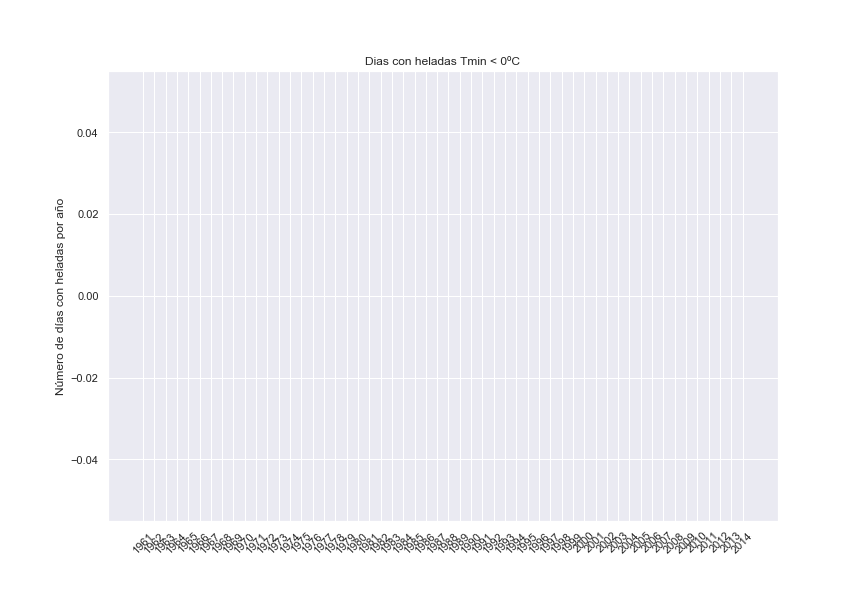
\includegraphics[scale=0.5]{FD.png}
\end{center} 
\begin{center}
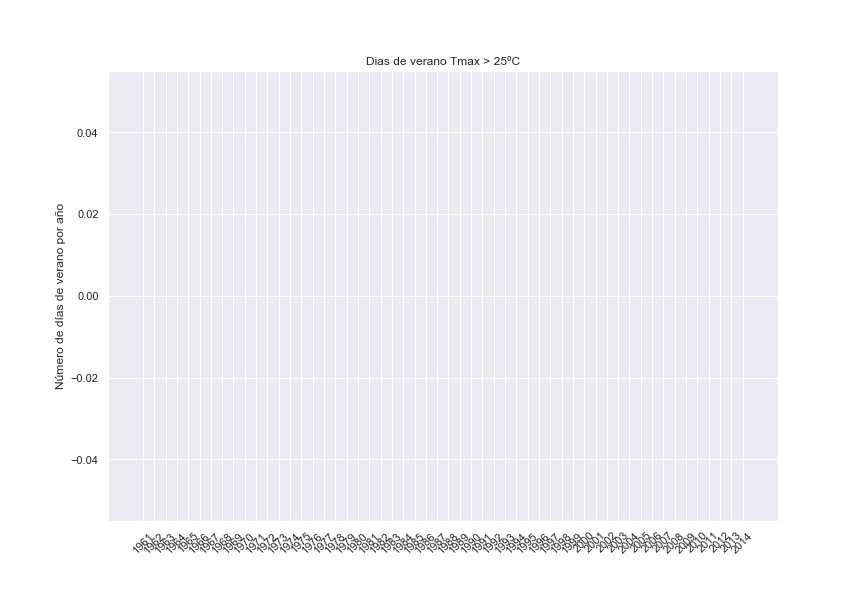
\includegraphics[scale=0.5]{SU.png}
\end{center} 
\begin{center}
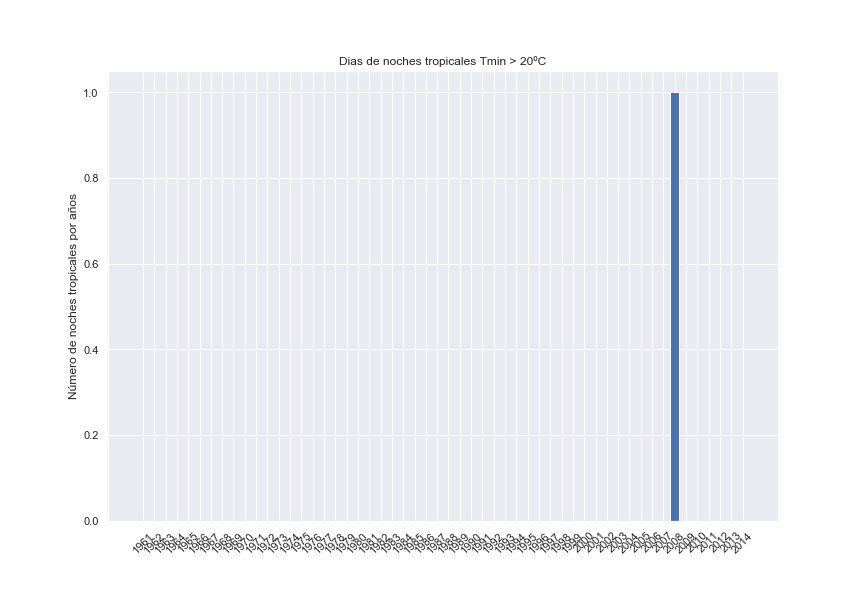
\includegraphics[scale=0.5]{FR.png}
\end{center} 
\begin{center}
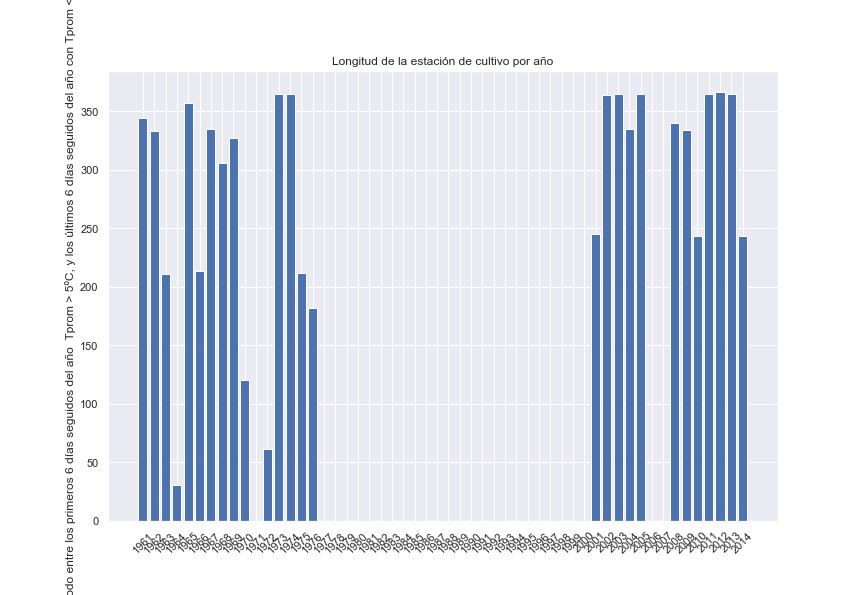
\includegraphics[scale=0.5]{GSL.png}
\end{center} 
\begin{center}
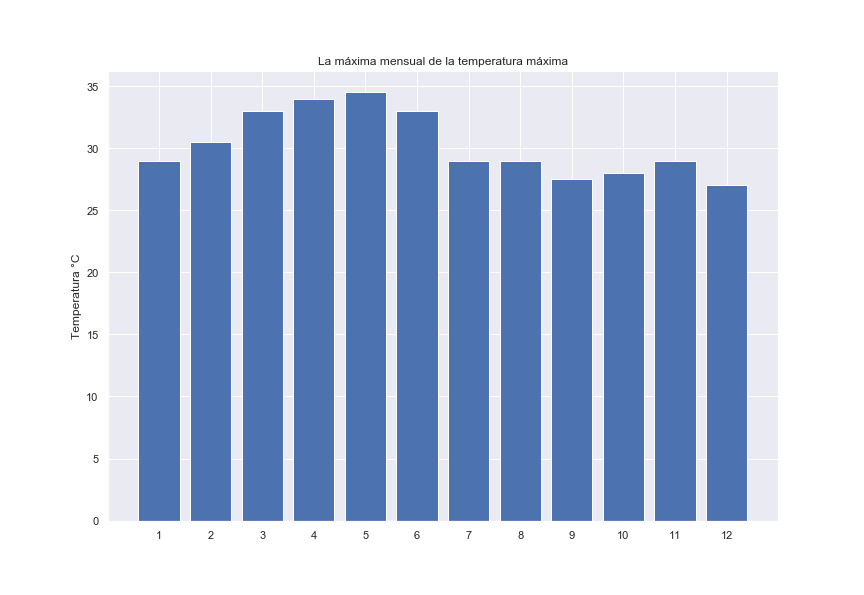
\includegraphics[scale=0.5]{TXx.png}
\end{center} 
\begin{center}
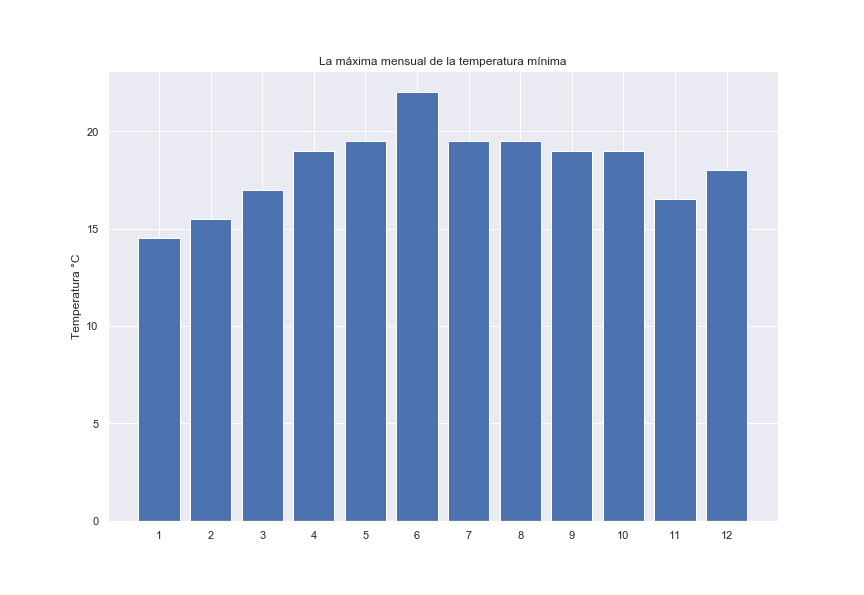
\includegraphics[scale=0.5]{TNx.png}
\end{center} 
\begin{center}
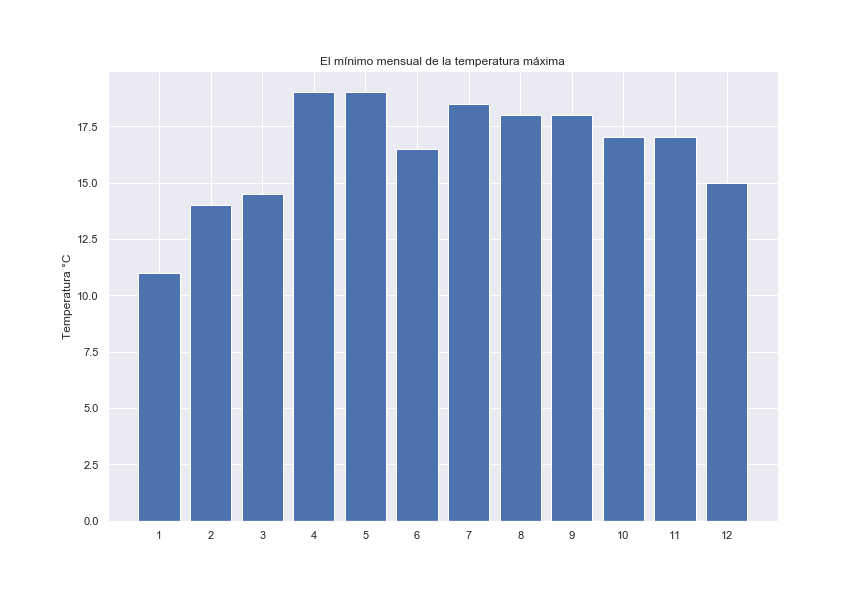
\includegraphics[scale=0.5]{TXn.png}
\end{center} 
\begin{center}
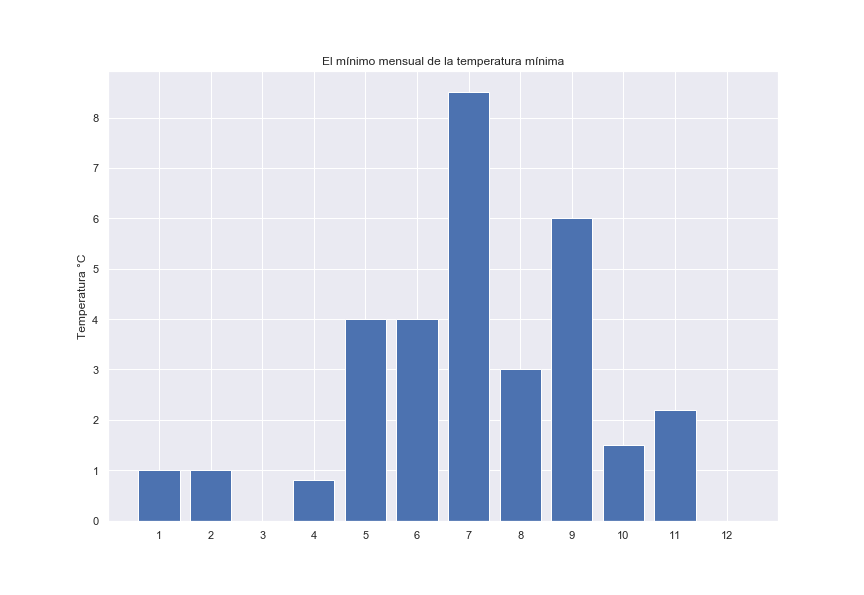
\includegraphics[scale=0.5]{TNn.png}
\end{center} 
\begin{center}
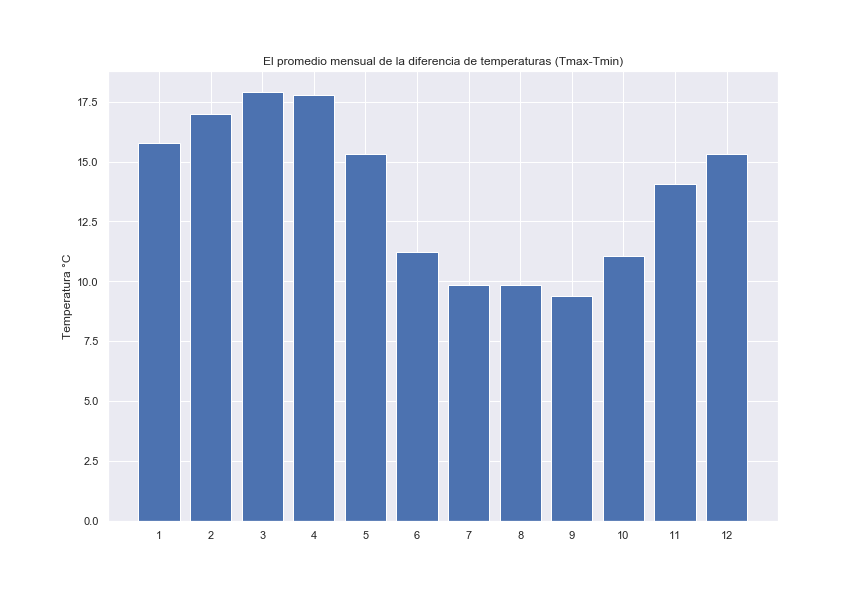
\includegraphics[scale=0.5]{DTR.png}
\end{center} 
\begin{center}
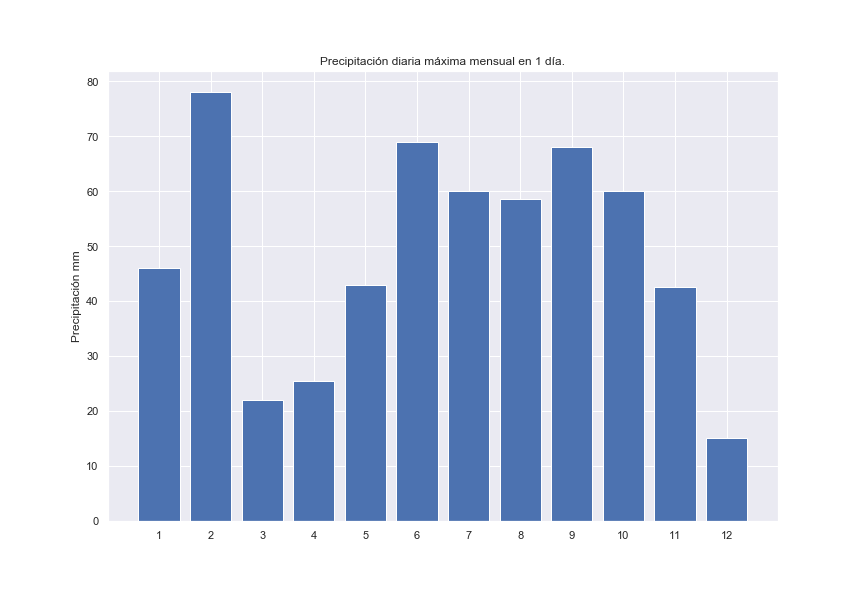
\includegraphics[scale=0.5]{Rx1day.png}
\end{center} 
\begin{center}
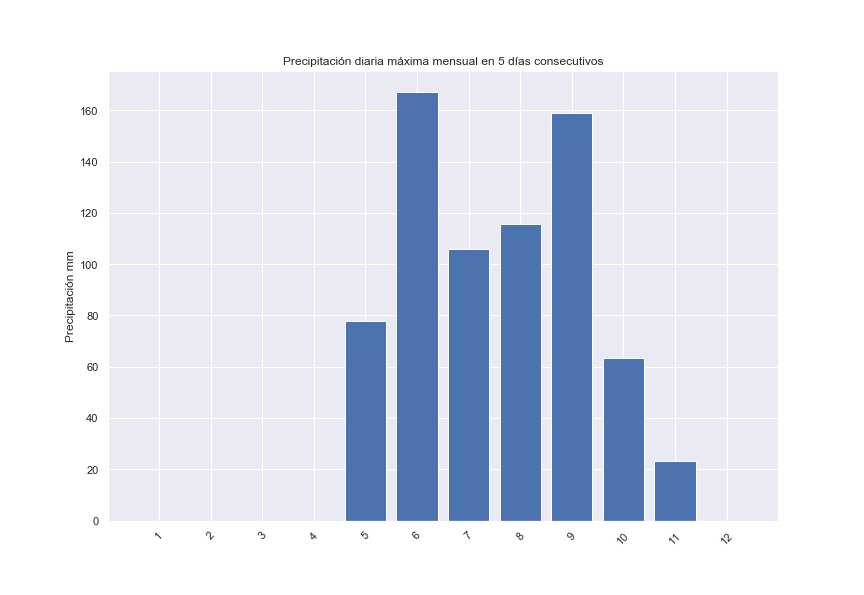
\includegraphics[scale=0.5]{Rx5day.png}
\end{center} 
\begin{center}
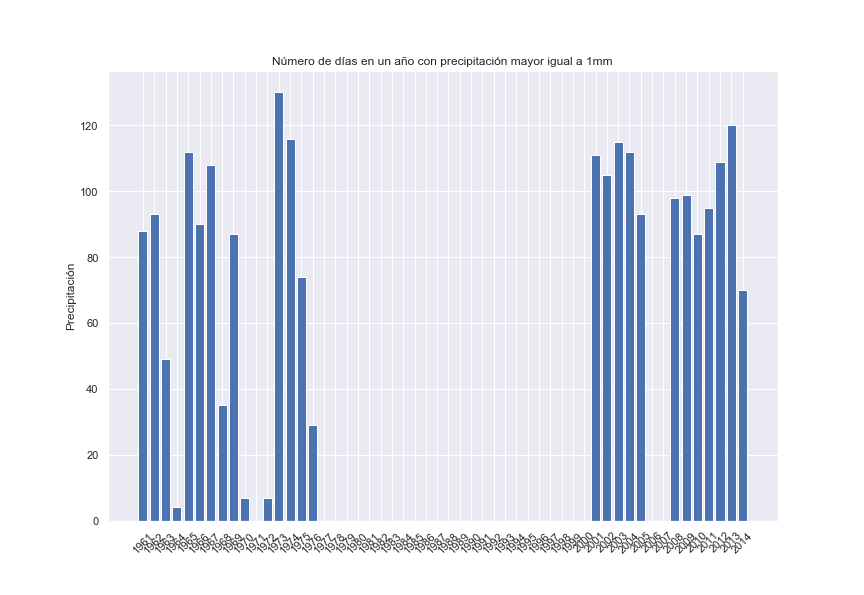
\includegraphics[scale=0.5]{SDII.png}
\end{center} 
\begin{center}
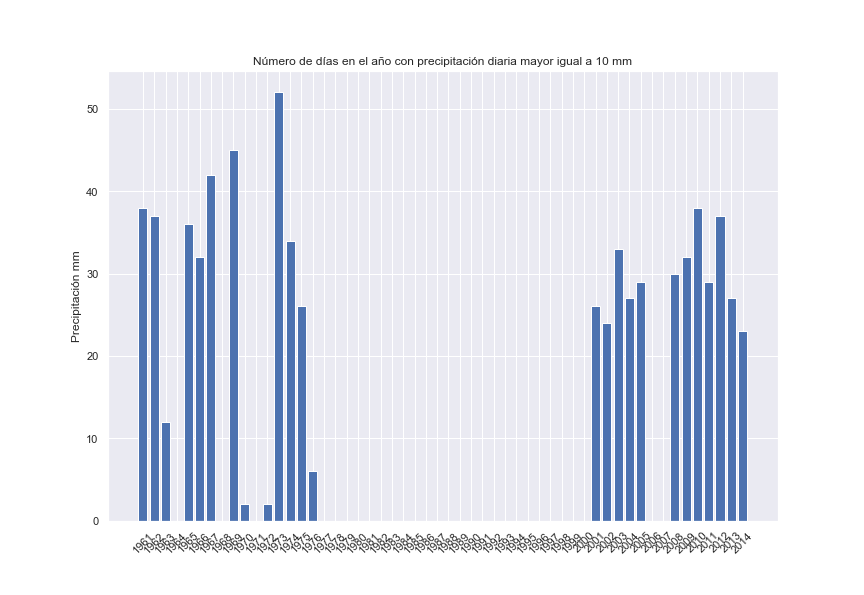
\includegraphics[scale=0.5]{R10mm.png}
\end{center} 
\begin{center}
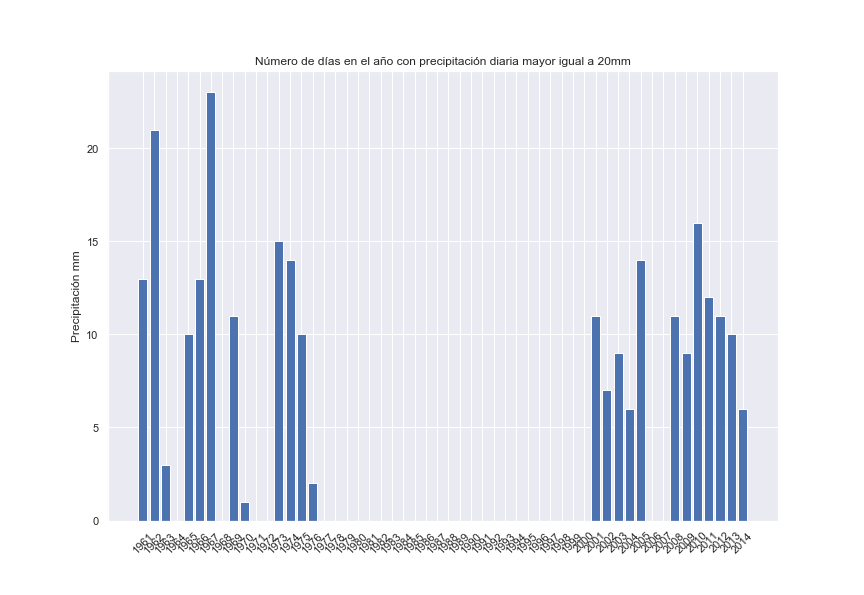
\includegraphics[scale=0.5]{R20mm.png}
\end{center} 
\begin{center}
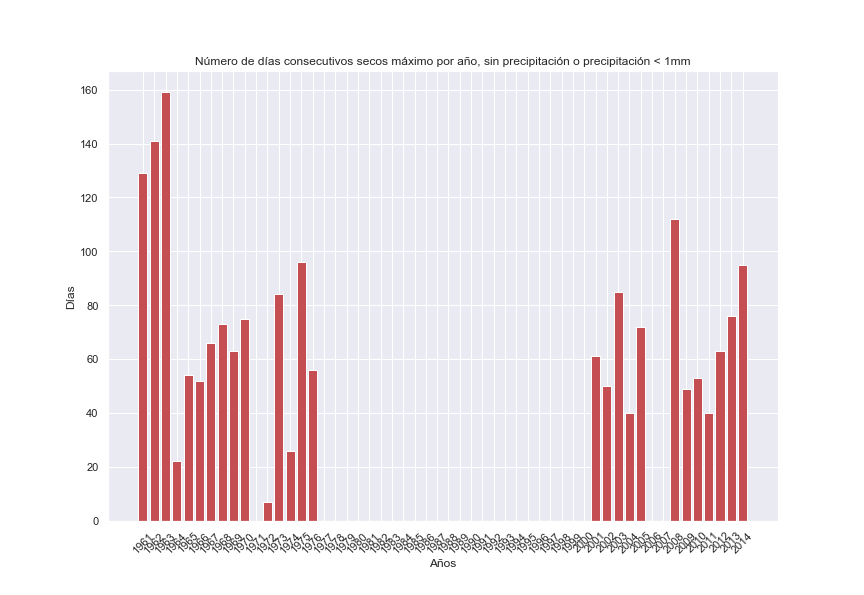
\includegraphics[scale=0.5]{CDD.png}
\end{center} 
\begin{center}
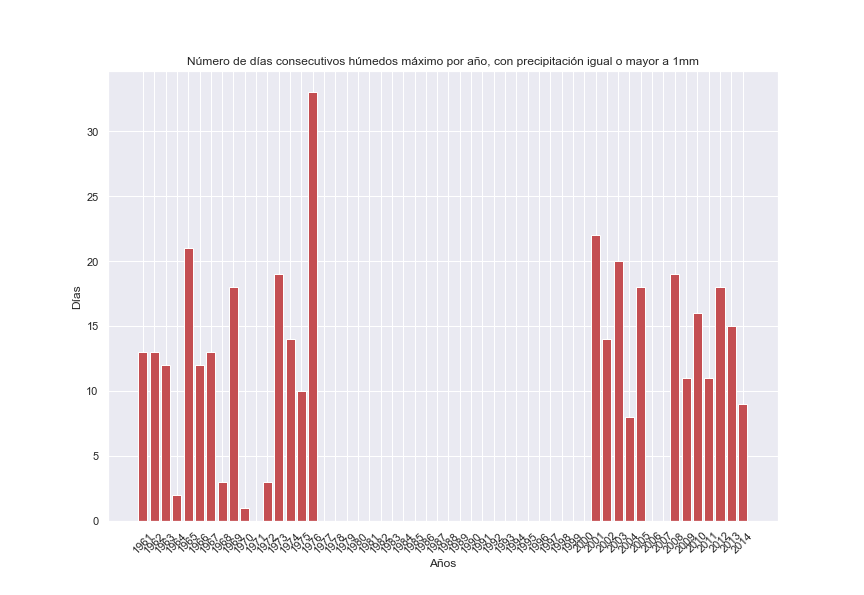
\includegraphics[scale=0.5]{CWD.png}
\end{center} 



\section{Conclusiones}
Podemos concluir que los indices son herramientas muy útiles para analizar mas detalladamente los datos y realizar un análisis de los mismos a partir de las gráficas, observamos diversos aspectos interesantes del municipio de Valle de Bravo con la información que nos proporciona la correspondiente estación del Servicio Meteorológico Nacional.

\section{Referencias}
\begin{itemize}
\item El Servicio Meteorológico Nacional, Información Estadística Climatológica,\\ Recuperado de:\\ https://smn.cna.gob.mx/es/climatologia/informacion-climatologica/informacion-estadistica-climatologica
\item Matplotlib. Recuperado de:\\ https://matplotlib.org/
\item Seaborn: statistical data visualization. Recuperado de:\\ https://seaborn.pydata.org/generated/seaborn.boxplot.html
\end{itemize}

\end{document}
